\documentclass[10pt]{beamer}
\usepackage{amsmath}
\usepackage{amssymb}
\usepackage{amsthm}
\usepackage{braket}
\usepackage{graphicx}
\usepackage{tikz}
\usepackage{algorithm}
\usepackage{algpseudocode}
\usepackage{multicol}
\usepackage{booktabs}
\usepackage{multirow}

\usetikzlibrary{positioning} % Added for proper positioning syntax

\usetheme{Madrid}
\usecolortheme{whale}
\setbeamertemplate{navigation symbols}{}
\setbeamertemplate{footline}{}

\title{\textbf{Rigorous Quantum Communication Framework}\\
\textbf{for Electromagnetic Signals in Optical Fibers}}
\subtitle{Cq Channel Capacity and Computational Hardness}
\author{Research Framework Integration}
\date{}

\begin{document}

\begin{frame}
\titlepage
\end{frame}

\begin{frame}{Outline}
\tableofcontents
\end{frame}

\section{Introduction and Motivation}

\begin{frame}{The Core Challenge}
\begin{block}{Problem Statement}
Develop a rigorous quantum communication framework for electromagnetic signals through optical fibers using Classical-Quantum (Cq) channel capacity, while simultaneously establishing the computational hardness of the associated signal inversion and decoding problems.
\end{block}

\begin{itemize}
\item \textbf{Physical Layer}: Maxwell's equations → quantum field theory
\item \textbf{Information Theory}: Cq channels and Holevo capacity
\item \textbf{Computational Complexity}: NP-hardness via SJIP reduction
\end{itemize}
\end{frame}

\begin{frame}{Why This Framework is Necessary}
\begin{columns}
\begin{column}{0.5\textwidth}
\textbf{Physical Necessity}
\begin{itemize}
\item Quantum nature of light
\item Non-commutative measurements
\item Physical parameter dependence
\end{itemize}

\textbf{Information-Theoretic Necessity}
\begin{itemize}
\item Holevo bound is fundamental
\item Optimal encoding/decoding
\end{itemize}
\end{column}

\begin{column}{0.5\textwidth}
\textbf{Computational Necessity}
\begin{itemize}
\item Decoding complexity: $O(M^N \cdot d^2)$
\item Measurement optimization: $d^N \times d^N$ matrices
\item Parameter optimization: $O(K \cdot M^N \cdot d^{3N})$
\end{itemize}

\textbf{Key Insight}
Understanding computational hardness guides practical approximations.
\end{column}
\end{columns}
\end{frame}

\begin{frame}{Framework Architecture: Integrated Approach}
\centering
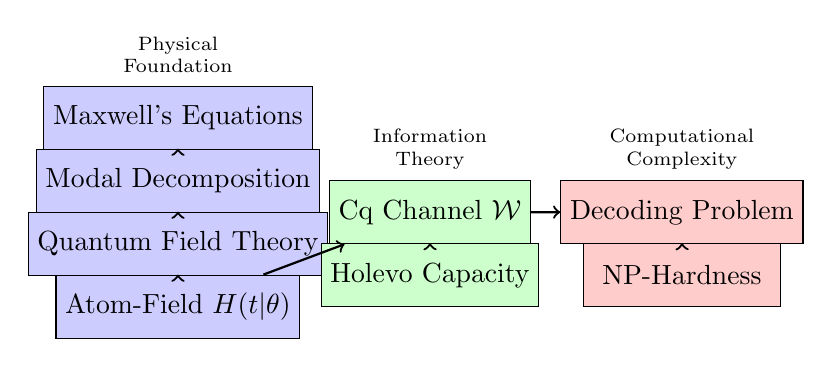
\begin{tikzpicture}[scale=0.8]
% Boxes
\node[draw, rectangle, minimum width=2.5cm, minimum height=0.8cm, fill=blue!20] (maxwell) at (0,5) {Maxwell's Equations};
\node[draw, rectangle, minimum width=2.5cm, minimum height=0.8cm, fill=blue!20] (modal) at (0,4) {Modal Decomposition};
\node[draw, rectangle, minimum width=2.5cm, minimum height=0.8cm, fill=blue!20] (quantum) at (0,3) {Quantum Field Theory};
\node[draw, rectangle, minimum width=2.5cm, minimum height=0.8cm, fill=blue!20] (hamiltonian) at (0,2) {Atom-Field $H(t|\theta)$};
\node[draw, rectangle, minimum width=2.5cm, minimum height=0.8cm, fill=green!20] (cq) at (4,3.5) {Cq Channel $\mathcal{W}$};
\node[draw, rectangle, minimum width=2.5cm, minimum height=0.8cm, fill=green!20] (holevo) at (4,2.5) {Holevo Capacity};
\node[draw, rectangle, minimum width=2.5cm, minimum height=0.8cm, fill=red!20] (decoding) at (8,3.5) {Decoding Problem};
\node[draw, rectangle, minimum width=2.5cm, minimum height=0.8cm, fill=red!20] (hardness) at (8,2.5) {NP-Hardness};

% Arrows
\draw[->, thick] (maxwell) -- (modal);
\draw[->, thick] (modal) -- (quantum);
\draw[->, thick] (quantum) -- (hamiltonian);
\draw[->, thick] (hamiltonian) -- (cq);
\draw[->, thick] (cq) -- (holevo);
\draw[->, thick] (cq) -- (decoding);
\draw[->, thick] (decoding) -- (hardness);

% Labels
\node[align=center, font=\scriptsize] at (0,6) {Physical\\Foundation};
\node[align=center, font=\scriptsize] at (4,4.5) {Information\\Theory};
\node[align=center, font=\scriptsize] at (8,4.5) {Computational\\Complexity};
\end{tikzpicture}
\end{frame}

\begin{frame}{How the Framework Works: 5 Layers}
\begin{enumerate}
\item \textbf{Layer 1: Electromagnetic Foundation}
\begin{itemize}
\item Maxwell's equations in inhomogeneous dielectric
\item Solve for fiber modes $E_m(r)$, $\beta_m(\omega)$
\item Include dispersion $\beta_2$, attenuation $\alpha$
\end{itemize}

\item \textbf{Layer 2: Quantum Description}
\begin{itemize}
\item Quantize field: $A(r,t) \to \hat{A}(r,t)$
\item Mode basis: $\hat{A} = \sum_m \sqrt{\frac{\hbar\omega_m}{2\epsilon_0 V}}(\hat{a}_m f_m + \text{h.c.})$
\item Hamiltonian: $H = \sum_m \hbar\omega_m \hat{a}_m^\dagger \hat{a}_m$
\end{itemize}
\end{enumerate}
\end{frame}

\begin{frame}{How the Framework Works (Continued)}
\begin{enumerate}
\setcounter{enumi}{2}
\item \textbf{Layer 3: Atom-Field Interaction}
\begin{itemize}
\item Two-level atoms: $H_{\text{atom}} = \hbar\omega_{eg}|e\rangle\langle e|$
\item Coupling: $V(t|\theta) = \hbar g(\theta)[\sigma_+ \hat{a} + \sigma_- \hat{a}^\dagger]$
\item Parameter dependence: $g(\theta) \propto 1/\sqrt{V_{\text{eff}}(\theta)}$
\end{itemize}

\item \textbf{Layer 4: Cq Channel Construction}
\begin{itemize}
\item Encoding: $x \mapsto \rho(x|\theta) = |\alpha_x\rangle\langle\alpha_x|$
\item Propagation: $\rho(x,L|\theta) = \mathcal{E}_{\text{fiber}}[\rho(x,0|\theta)]$
\item Measurement: $p(y|x) = \text{Tr}[\Pi_y \rho(x,L|\theta)]$
\end{itemize}

\item \textbf{Layer 5: Optimization \& Complexity}
\begin{itemize}
\item Maximize: $C(\theta) = \max_{p(x)} \chi(\{p(x), \rho(x|\theta)\})$
\item Subject to: Physical constraints on $\theta$
\item Prove: Decoding is NP-hard via SJIP reduction
\end{itemize}
\end{enumerate}
\end{frame}

\section{Electromagnetic Field Propagation}

\begin{frame}{Maxwell's Equations in Optical Fibers}
\begin{block}{In Dielectric Medium with $\epsilon(r)$}
\begin{columns}
\begin{column}{0.45\textwidth}
\begin{align*}
\nabla \cdot \mathbf{D} &= \rho_{\text{free}} \\
\nabla \cdot \mathbf{B} &= 0 \\
\nabla \times \mathbf{E} &= -\frac{\partial \mathbf{B}}{\partial t} \\
\nabla \times \mathbf{H} &= \mathbf{J}_{\text{free}} + \frac{\partial \mathbf{D}}{\partial t}
\end{align*}
\end{column}
\begin{column}{0.45\textwidth}
\begin{align*}
\mathbf{D} &= \epsilon(r)\mathbf{E} \\
\mathbf{B} &= \mu_0\mathbf{H} \\
n(r) &= \sqrt{\epsilon_r(r)}
\end{align*}
\end{column}
\end{columns}
\end{block}

\begin{block}{Step-Index Fiber Geometry}
\begin{equation*}
n(r) = \begin{cases}
n_{\text{core}} & r < a \ (\text{core}) \\
n_{\text{clad}} & r > a \ (\text{cladding})
\end{cases}
\end{equation*}
\end{block}
\end{frame}

\begin{frame}{Fiber Parameters and Modal Decomposition}
\begin{columns}
\begin{column}{0.5\textwidth}
\textbf{Key Parameters}
\begin{align*}
\text{NA} &= \sqrt{n_{\text{core}}^2 - n_{\text{clad}}^2} \\
V &= \frac{2\pi a}{\lambda_0}\text{NA} \\
\Delta &= \frac{n_{\text{core}} - n_{\text{clad}}}{n_{\text{core}}}
\end{align*}

\textbf{Single-mode condition:} $V < 2.405$
\end{column}

\begin{column}{0.5\textwidth}
\textbf{Modal Expansion}
\begin{equation*}
\mathbf{E}(r,\phi,z,t) = \sum_m a_m \mathbf{E}_m(r,\phi) e^{i(\beta_m z - \omega t)} + \text{c.c.}
\end{equation*}

\textbf{LP$_{01}$ Mode}
\begin{equation*}
E_{01}(r) \propto \begin{cases}
J_0(ur/a) & r < a \\
\frac{J_0(u)}{K_0(w)}K_0(wr/a) & r > a
\end{cases}
\end{equation*}
\end{column}
\end{columns}

\begin{block}{Eigenvalue Equation}
\begin{equation*}
\frac{u J_1(u)}{J_0(u)} = \frac{w K_1(w)}{K_0(w)}, \quad u^2 + w^2 = V^2
\end{equation*}
\end{block}
\end{frame}

\begin{frame}{Dispersion in Optical Fibers}
\begin{block}{Propagation Constant Expansion}
\begin{equation*}
\beta(\omega) = \beta_0 + \beta_1(\omega - \omega_0) + \frac{\beta_2}{2}(\omega - \omega_0)^2 + \frac{\beta_3}{6}(\omega - \omega_0)^3 + \cdots
\end{equation*}
\end{block}

\begin{columns}
\begin{column}{0.5\textwidth}
\textbf{Physical Meaning}
\begin{align*}
\beta_0 &= \beta(\omega_0) \\
\beta_1 &= \frac{1}{v_g} \ \text{(inverse group velocity)} \\
\beta_2 &= \text{GVD coefficient} \\
D &= -\frac{2\pi c}{\lambda_0^2}\beta_2
\end{align*}
\end{column}

\begin{column}{0.5\textwidth}
\textbf{Numerical Values}
\begin{itemize}
\item $D \approx 17$ ps/(nm·km) at 1550 nm
\item $\beta_2 \approx -21.7$ ps$^2$/km
\item $\alpha_{\text{dB}} \approx 0.2$ dB/km
\end{itemize}
\end{column}
\end{columns}

\begin{block}{Dispersion Length}
\begin{equation*}
L_D = \frac{T_0^2}{|\beta_2|}, \quad T(z) = T_0\sqrt{1 + \left(\frac{z}{L_D}\right)^2}
\end{equation*}
\end{block}
\end{frame}

\section{Quantum Field Theory in Fibers}

\begin{frame}{Quantization Procedure}
\begin{block}{Field Operator}
\begin{equation*}
\hat{\mathbf{A}}(r,t) = \sum_m \sqrt{\frac{\hbar\omega_m}{2\epsilon_0 \epsilon_m V_m}}\left[\hat{a}_m(t) \mathbf{f}_m(r) + \hat{a}_m^\dagger(t) \mathbf{f}_m^*(r)\right]
\end{equation*}
\end{block}

\begin{columns}
\begin{column}{0.5\textwidth}
\textbf{Commutation Relations}
\begin{equation*}
[\hat{a}_m, \hat{a}_n^\dagger] = \delta_{mn}
\end{equation*}

\textbf{Hamiltonian}
\begin{equation*}
\hat{H}_{\text{field}} = \sum_m \hbar\omega_m\left(\hat{a}_m^\dagger \hat{a}_m + \frac{1}{2}\right)
\end{equation*}
\end{column}

\begin{column}{0.5\textwidth}
\textbf{Coherent States}
\begin{equation*}
\hat{a}_m|\alpha_m\rangle = \alpha_m|\alpha_m\rangle
\end{equation*}

\textbf{Propagation}
\begin{equation*}
\alpha(L) = \alpha(0) \exp[i\beta(\omega)L]\exp[-\alpha L/2]
\end{equation*}
\end{column}
\end{columns}

\begin{block}{Density Matrix Evolution}
\begin{equation*}
\hat{\rho}(L) = |\alpha(L)\rangle\langle\alpha(L)| = \hat{U}(L)\hat{\rho}(0)\hat{U}^\dagger(L)
\end{equation*}
\end{block}
\end{frame}

\begin{frame}{Atom-Field Interaction Hamiltonian $H(t|\theta)$}
\begin{block}{Total Hamiltonian}
\begin{equation*}
H(t|\theta) = H_0 + V(t|\theta)
\end{equation*}
\end{block}

\begin{columns}
\begin{column}{0.45\textwidth}
\textbf{Free Hamiltonian}
\begin{align*}
H_0 &= H_{\text{atom}} + H_{\text{field}} \\
H_{\text{atom}} &= \hbar\omega_{eg}|e\rangle\langle e|
\end{align*}

\textbf{Interaction (RWA)}
\begin{equation*}
V_I(\theta) = \hbar g(\theta)[\sigma_+ \hat{a} + \sigma_- \hat{a}^\dagger]
\end{equation*}
\end{column}

\begin{column}{0.55\textwidth}
\textbf{Coupling Strength}
\begin{equation*}
g(\theta) = d_{eg}\sqrt{\frac{\omega_0^3}{2\hbar\epsilon_0 V_{\text{eff}}(\theta)}}|f_0(r_{\text{atom}}|\theta)|
\end{equation*}

\textbf{Parameter Dependence}
\begin{align*}
V_{\text{eff}}(\theta) &\sim \pi a^2(\theta) L_{\text{eff}} \\
g(a) &\propto 1/a \ \text{(smaller core → stronger coupling)}
\end{align*}
\end{column}
\end{columns}
\end{frame}

\begin{frame}{Master Equation with Dissipation}
\begin{block}{Lindblad Master Equation}
\begin{equation*}
\frac{d\hat{\rho}}{dt} = -\frac{i}{\hbar}[H(t|\theta), \hat{\rho}] + \mathcal{L}_{\text{spont}} + \mathcal{L}_{\text{loss}}
\end{equation*}
\end{block}

\begin{columns}
\begin{column}{0.5\textwidth}
\textbf{Spontaneous Emission}
\begin{equation*}
\mathcal{L}_{\text{spont}} = \gamma\left(\sigma_- \hat{\rho}\sigma_+ - \frac{1}{2}\{\sigma_+\sigma_-, \hat{\rho}\}\right)
\end{equation*}

\textbf{Photon Loss}
\begin{equation*}
\kappa = \frac{\alpha(\theta)v_g}{2}
\end{equation*}
\end{column}

\begin{column}{0.5\textwidth}
\textbf{Loss Term}
\begin{equation*}
\mathcal{L}_{\text{loss}} = \kappa\left(\hat{a}\hat{\rho}\hat{a}^\dagger - \frac{1}{2}\{\hat{a}^\dagger\hat{a}, \hat{\rho}\}\right)
\end{equation*}

\textbf{Typical Values}
\begin{itemize}
\item $\gamma \approx 10^8$ s$^{-1}$ (atomic)
\item $\kappa \approx 0.046$ km$^{-1}$ (fiber)
\end{itemize}
\end{column}
\end{columns}
\end{frame}

\section{Cq Channel Theory}

\begin{frame}{Classical-Quantum Channel Definition}
\begin{block}{Encoding Map}
\begin{equation*}
\mathcal{W}: \mathcal{X} \to \mathcal{S}(\mathcal{H}), \quad x \mapsto \rho(x|\theta)
\end{equation*}
\end{block}

\begin{columns}
\begin{column}{0.5\textwidth}
\textbf{Components}
\begin{itemize}
\item Alphabet: $\mathcal{X} = \{x_1, \ldots, x_M\}$
\item Density operators: $\rho(x)^\dagger = \rho(x)$, $\rho(x) \geq 0$, $\text{Tr}[\rho(x)] = 1$
\item Parameters: $\theta = \{L, \alpha, \beta_2, a, \ldots\}$
\end{itemize}
\end{column}

\begin{column}{0.5\textwidth}
\textbf{Example: BPSK}
\begin{align*}
x=0 &: \rho(0|\theta) = |\alpha(\theta)\rangle\langle\alpha(\theta)| \\
x=1 &: \rho(1|\theta) = |-\alpha(\theta)\rangle\langle-\alpha(\theta)|
\end{align*}
\begin{equation*}
\alpha(\theta) = \alpha_0 e^{i\beta(\theta)L}e^{-\alpha(\theta)L/2}
\end{equation*}
\end{column}
\end{columns}

\begin{block}{N-Symbol Transmission}
\begin{equation*}
\rho(x_1, \ldots, x_N|\theta) = \bigotimes_{i=1}^N \rho(x_i|\theta)
\end{equation*}
Hilbert space: $\dim(\mathcal{H}^{\otimes N}) = (\dim \mathcal{H})^N$
\end{block}
\end{frame}

\begin{frame}{Receiver Measurement and Holevo Capacity}
\begin{block}{POVM Measurement}
\begin{equation*}
\Pi_y \geq 0, \quad \sum_y \Pi_y = I, \quad p(y|x,\theta) = \text{Tr}[\Pi_y \rho(x|\theta)]
\end{equation*}
\end{block}

\begin{columns}
\begin{column}{0.5\textwidth}
\textbf{Holevo Quantity}
\begin{equation*}
\chi(\{p(x), \rho(x|\theta)\}) = S(\bar{\rho}) - \sum_x p(x)S(\rho(x|\theta))
\end{equation*}
\begin{align*}
\bar{\rho} &= \sum_x p(x)\rho(x|\theta) \\
S(\rho) &= -\text{Tr}[\rho\log\rho]
\end{align*}
\end{column}

\begin{column}{0.5\textwidth}
\textbf{Holevo Bound}
\begin{equation*}
I(X:Y) \leq \chi(\{p(x), \rho(x|\theta)\})
\end{equation*}

\textbf{Channel Capacity}
\begin{equation*}
C(\theta) = \max_{p(x)} \chi(\{p(x), \rho(x|\theta)\})
\end{equation*}
\end{column}
\end{columns}

\begin{block}{Achievability}
Holevo-Schumacher-Westmoreland theorem: $\chi$ is achievable with collective measurements.
\end{block}
\end{frame}

\section{Decoding and Inversion Problems}




\begin{frame}{Signal Flow and Computational Bottlenecks}
\centering
\textbf{Signal Flow:}

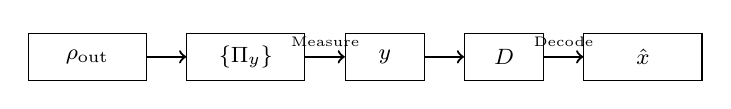
\begin{tikzpicture}[node distance=0.5cm]
% Nodes - smaller sizes
\node[draw, rectangle, minimum width=1.5cm, minimum height=0.6cm, font=\footnotesize] (output) {$\rho_{\text{out}}$};
\node[draw, rectangle, minimum width=1.5cm, minimum height=0.6cm, font=\footnotesize, right=of output] (measure) {$\{\Pi_y\}$};
\node[draw, rectangle, minimum width=1cm, minimum height=0.6cm, font=\footnotesize, right=of measure] (result) {$y$};
\node[draw, rectangle, minimum width=1cm, minimum height=0.6cm, font=\footnotesize, right=of result] (decode) {$D$};
\node[draw, rectangle, minimum width=1.5cm, minimum height=0.6cm, font=\footnotesize, right=of decode] (estimate) {$\hat{x}$};

% Arrows
\draw[->, thick] (output) -- (measure);
\draw[->, thick] (measure) -- node[above, font=\tiny] {Measure} (result);
\draw[->, thick] (result) -- (decode);
\draw[->, thick] (decode) -- node[above, font=\tiny] {Decode} (estimate);
\end{tikzpicture}

\vspace{0.3cm}

\begin{columns}
\begin{column}{0.48\textwidth}
\begin{alertblock}{Problem 1: DECODING}
Given $y$, infer $x$\\
Complexity: $O(M^N \cdot d^2)$
\end{alertblock}
\end{column}
\begin{column}{0.48\textwidth}
\begin{alertblock}{Problem 2: INVERSION}
Design optimal $\{\Pi_y\}$ and $D$\\
NP-hard optimization
\end{alertblock}
\end{column}
\end{columns}
\end{frame}



\begin{frame}{Decoding Problem Definition}
\begin{block}{Formal Definition}
\textbf{Given:}
\begin{itemize}
\item Prior $p(x)$ over $\mathcal{X}^N$
\item Encoding states $\{\rho(x|\theta)\}$ for $x \in \mathcal{X}^N$
\item POVM $\{\Pi_y\}$ with $\sum_y \Pi_y = I$
\item Observed outcome $y$
\end{itemize}

\textbf{Find:} $\hat{x}$ minimizing
\begin{equation*}
P_{\text{error}} = \Pr[\hat{x} \neq x] = \sum_x p(x)\sum_{y:D(y)\neq x} \text{Tr}[\Pi_y\rho(x|\theta)]
\end{equation*}
\end{block}

\begin{columns}
\begin{column}{0.5\textwidth}
\textbf{MAP Decoder}
\begin{equation*}
\hat{x}_{\text{MAP}}(y) = \arg\max_x p(x)\text{Tr}[\Pi_y\rho(x|\theta)]
\end{equation*}
\end{column}

\begin{column}{0.5\textwidth}
\textbf{ML Decoder (uniform prior)}
\begin{equation*}
\hat{x}_{\text{ML}}(y) = \arg\max_x \text{Tr}[\Pi_y\rho(x|\theta)]
\end{equation*}
\end{column}
\end{columns}
\end{frame}

\begin{frame}{Computational Complexity Analysis}
\begin{block}{Problem Dimensions}
\begin{itemize}
\item Alphabet size: $M$
\item Sequence length: $N$
\item Total messages: $|\mathcal{X}^N| = M^N$
\item Hilbert space dimension: $d = \dim(\mathcal{H}^{\otimes N}) = (\dim\mathcal{H})^N$
\end{itemize}
\end{block}

\begin{example}[Binary System]
$M = 2$, $N = 100$, qubit encoding ($d = 2$):
\begin{align*}
\text{Total messages} &: 2^{100} \approx 10^{30} \\
\text{Hilbert space} &: 2^{100} \text{ dimensions} \\
\text{Trace computation} &: O(2^{200}) \ \text{operations}
\end{align*}
Clearly intractable!
\end{example}
\end{frame}

\begin{frame}
\begin{block}{Naive MAP Decoding Complexity}
\begin{equation*}
O(M^N \cdot d^2) \ \text{operations}
\end{equation*}
Exponential in both $N$ and $\log d$!
\end{block}
\end{frame}

\section{NP-Hardness via SJIP Reduction}

\begin{frame}{Semigroup Julia Inversion Problem (SJIP)}
\begin{definition}[SJIP]
\textbf{Given:}
\begin{itemize}
\item Semigroup $G$ with operation $\cdot$
\item Element $y \in G$
\item Finite subset $S \subseteq G$
\end{itemize}
\textbf{Determine:} Whether $\exists S' \subseteq S$ such that
\begin{equation*}
\prod_{x \in S'} x = y
\end{equation*}
\end{definition}

\begin{block}{Complexity Status}
\begin{itemize}
\item Generalizes Subset-Sum problem
\item Natural encoding in quantum systems
\end{itemize}
\end{block}
\end{frame}

\begin{frame}{Reduction from Subset-Sum to SJIP}
\begin{theorem}[NP-Hardness of SJIP]
SJIP is NP-hard via polynomial-time reduction from Subset-Sum.
\end{theorem}

\begin{proof}[Proof Sketch]
\begin{enumerate}
\item \textbf{Subset-Sum Instance:} $A = \{a_1, \ldots, a_n\}$, target $T$
\item \textbf{Construct SJIP Instance:}
\begin{itemize}
\item $G = (\mathbb{Z}, +)$ (additive integers)
\item $S = A$
\item $y = T$
\end{itemize}
\item \textbf{Correctness:} $\exists S' \subseteq S$ with $\sum_{x \in S'} x = T$ iff Subset-Sum solution exists
\item \textbf{Polynomial-Time:} Reduction takes $O(n)$ time
\end{enumerate}
Thus, Subset-Sum $\leq_p$ SJIP $\Rightarrow$ SJIP is NP-hard.
\end{proof}
\end{frame}

\begin{frame}{Connection to Quantum Decoding}
\begin{theorem}[Reduction from SJIP to Quantum Decoding]
The quantum decoding problem for Cq channels with coherent states is at least as hard as SJIP.
\end{theorem}

\begin{proof}[Encoding Strategy]
\begin{enumerate}
\item Let $G = (\mathbb{C}, \times)$ (multiplicative complex numbers)
\item Encode each $x_i \in S$ as coherent state: $|x_i\rangle = |\alpha_i\rangle$ with $\alpha_i = x_i$
\item Measurement outcome $y$ corresponds to product
\item Decoding problem: Determine if $\exists S' \subseteq S$ such that $\prod_{x \in S'} x = y$
\end{enumerate}
This exactly embeds SJIP into quantum decoding.
\end{proof}

\begin{corollary}[Hardness of Optimal Decoding]
For any quantum communication system with $M \geq 2$, $N \geq 2$, optimal decoding is NP-hard.
\end{corollary}
\end{frame}

\section{Implications and Applications}

\begin{frame}{Fundamental Limits and Practical Consequences}
\begin{columns}
\begin{column}{0.5\textwidth}
\textbf{Fundamental Limits}
\begin{itemize}
\item Optimal decoding is NP-hard
\item Exact capacity computation is intractable
\item Optimal measurement design is NP-hard
\end{itemize}

\textbf{Practical Approximations}
\begin{itemize}
\item Belief propagation: $O(MN)$
\item Tensor networks: $O(N\chi^3)$
\item Machine learning: $O(KN^2)$
\end{itemize}
\end{column}

\begin{column}{0.5\textwidth}
\textbf{Parameter Optimization}
\begin{equation*}
\max_{\theta} C(\theta) = \max_{\theta} \max_{p(x)} \chi(\{p(x), \rho(x|\theta)\})
\end{equation*}
Double optimization:
\begin{enumerate}
\item Inner loop: Compute $\chi$ (NP-hard)
\item Outer loop: Optimize $\theta$ (non-convex)
\end{enumerate}
\end{column}
\end{columns}

\begin{block}{Engineering Guidance}
\begin{itemize}
\item Use approximations with provable bounds
\item Design systems knowing fundamental limits
\item Focus on practically implementable schemes
\end{itemize}
\end{block}
\end{frame}

\begin{frame}{Fiber Parameter Dependencies}
\begin{columns}
\begin{column}{0.33\textwidth}
\textbf{Core Radius}
\begin{equation*}
g(a) \propto \frac{1}{a}
\end{equation*}
\begin{equation*}
C(a) \approx C_0 \left(1 - e^{-\kappa/a^2}\right)
\end{equation*}
\end{column}

\begin{column}{0.33\textwidth}
\textbf{Propagation Distance}
\begin{equation*}
C(L) = C_0 e^{-\alpha L} \cdot \frac{1}{\sqrt{1 + (L/L_D)^2}}
\end{equation*}
\end{column}

\begin{column}{0.33\textwidth}
\textbf{Temperature}
\begin{equation*}
\frac{dn}{dT} \approx 10^{-5} \ \text{K}^{-1}
\end{equation*}
\begin{equation*}
\frac{dC}{dT} \approx -\gamma C
\end{equation*}
\end{column}
\end{columns}

\begin{block}{Physical Constraints}
\begin{itemize}
\item $a \geq a_{\text{min}}$ (manufacturing limits)
\item $L \leq L_{\text{max}}$ (attenuation limit)
\item $T_{\text{min}} \leq T \leq T_{\text{max}}$ (operating range)
\end{itemize}
\end{block}
\end{frame}

\begin{frame}{Algorithmic Solutions}
\begin{columns}
\begin{column}{0.5\textwidth}
\begin{algorithm}[H]
\caption{Approximate Quantum Decoding}
\begin{algorithmic}[1]
\Require $\rho$, $\{\rho_x\}$, $\epsilon$
\Ensure $\hat{x}$
\State $\mathbf{b} \leftarrow \mathbf{1}/M$
\For{$t = 1$ to $T_{\max}$}
\For{each $x$}
\State $L_x \leftarrow \text{Tr}[\rho \rho_x]$
\State $b_x \leftarrow b_x \cdot L_x$
\EndFor
\State Normalize $\mathbf{b}$
\If{$\max_x b_x > 1 - \epsilon$}
\State \Return $\arg\max_x b_x$
\EndIf
\EndFor
\State \Return $\arg\max_x b_x$
\end{algorithmic}
\end{algorithm}
\end{column}

\begin{column}{0.5\textwidth}
\begin{algorithm}[H]
\caption{Fiber Parameter Optimization}
\begin{algorithmic}[1]
\Require $\theta_0$, $C(\theta)$, $\eta$
\Ensure $\theta^*$
\State $\theta \leftarrow \theta_0$
\For{$k = 1$ to $K$}
\State $\nabla C \leftarrow \text{EstimateGradient}(\theta)$
\State $\theta \leftarrow \theta + \eta \nabla C$
\State $\theta \leftarrow \text{ProjectToFeasible}(\theta)$
\EndFor
\State \Return $\theta$
\end{algorithmic}
\end{algorithm}

\textbf{Complexity:}
\begin{itemize}
\item Gradient estimation: $O(K \cdot \text{poly}(N))$
\item Each iteration: Polynomial in system size
\end{itemize}
\end{column}
\end{columns}
\end{frame}

\section{Conclusion and Future Work}

\begin{frame}{Key Contributions Summary}
\begin{enumerate}
\item \textbf{Integrated Framework}
\begin{itemize}
\item Unified physical, information-theoretic, computational approach
\item Maxwell → quantum → information → complexity
\end{itemize}

\item \textbf{Explicit Parameter Dependence}
\begin{itemize}
\item $g(\theta)$, $\alpha(\theta)$, $\beta_2(\theta)$ in terms of fiber geometry
\item Engineering-ready formulas
\end{itemize}

\item \textbf{Complexity Analysis}
\begin{itemize}
\item Proved NP-hardness via SJIP reduction
\item Explained why optimal decoding is intractable
\end{itemize}

\item \textbf{Practical Formulas}
\begin{itemize}
\item Capacity expressions $C(\theta)$
\item Design guidelines and approximations
\end{itemize}
\end{enumerate}
\end{frame}

\begin{frame}{Future Research Directions}
\begin{columns}
\begin{column}{0.5\textwidth}
\textbf{Algorithmic Approximations}
\begin{itemize}
\item Polynomial-time algorithms with bounds
\item Quantum-inspired classical algorithms
\item Near-optimal practical decoders
\end{itemize}

\textbf{Experimental Validation}
\begin{itemize}
\item Test predictions against experiments
\item Measure $C(\theta)$ vs. parameters
\item Real-system validation
\end{itemize}
\end{column}

\begin{column}{0.5\textwidth}
\textbf{Extensions}
\begin{itemize}
\item Nonlinear effects ($\chi^{(3)}$)
\item Multi-mode fibers (MDM)
\item Quantum key distribution
\item Quantum networks
\end{itemize}

\textbf{Theoretical Developments}
\begin{itemize}
\item Tighter complexity bounds
\item Quantum advantage proofs
\item New capacity theorems
\end{itemize}
\end{column}
\end{columns}
\end{frame}

\begin{frame}{Final Remarks: A Complete Picture}
\begin{block}{Framework Provides:}
\begin{enumerate}
\item \textbf{Physical Foundation:} Rigorous from Maxwell to quantum
\item \textbf{Information-Theoretic Limits:} Holevo capacity as fundamental bound
\item \textbf{Computational Reality:} NP-hardness explains practical difficulties
\item \textbf{Engineering Guidance:} Explicit dependencies for system design
\end{enumerate}
\end{block}

\begin{block}{The Complete Marriage}
Physical modeling + Information theory + Computational complexity = Complete understanding of quantum fiber-optic communication systems.
\end{block}

\begin{center}
\Large \textbf{Thank You! Questions?}
\end{center}
\end{frame}

\begin{frame}{Mathematical Appendix I: Physical Foundations}
\footnotesize

\textbf{Maxwell's Equations (Dielectric)}
\begin{align*}
\nabla \cdot \mathbf{D} &= \rho_{\text{free}} \\
\nabla \cdot \mathbf{B} &= 0 \\
\nabla \times \mathbf{E} &= -\frac{\partial \mathbf{B}}{\partial t} \\
\nabla \times \mathbf{H} &= \mathbf{J}_{\text{free}} + \frac{\partial \mathbf{D}}{\partial t}
\end{align*}

\textbf{Fiber Mode Equation}
\begin{equation*}
\frac{d^2R}{dr^2} + \frac{1}{r}\frac{dR}{dr} + \left(k_0^2n^2(r) - \beta^2 - \frac{m^2}{r^2}\right)R = 0
\end{equation*}

\textbf{Quantization in Fibers}
\begin{equation*}
\hat{\mathbf{A}}(r,t) = \sum_m \sqrt{\frac{\hbar\omega_m}{2\epsilon_0 \epsilon_m V_m}}[\hat{a}_m(t) \mathbf{f}_m(r) + \hat{a}_m^\dagger(t) \mathbf{f}_m^*(r)]
\end{equation*}

\textbf{Coupling Strength}
\begin{equation*}
g(\theta) = d_{eg}\sqrt{\frac{\omega_0^3}{2\hbar\epsilon_0 V_{\text{eff}}(\theta)}}
\end{equation*}

\end{frame}


\begin{frame}{Mathematical Appendix II: Information Theory}
\footnotesize

\textbf{Holevo Quantity}
\begin{equation*}
\chi(\{p(x), \rho(x|\theta)\}) = S(\bar{\rho}) - \sum_x p(x)S(\rho(x|\theta))
\end{equation*}

\textbf{Channel Capacity}
\begin{equation*}
C(\theta) = \max_{p(x)} \chi(\{p(x), \rho(x|\theta)\})
\end{equation*}

\textbf{BPSK with Coherent States}
\begin{align*}
C &= \max_{0 \leq p \leq 1} \left[ H_2\left(\frac{1 + \sqrt{1 - e^{-4|\alpha|^2}}}{2}\right) - H_2(p) \right] \\
H_2(x) &= -x\log x - (1-x)\log(1-x)
\end{align*}

\textbf{Dispersion and Attenuation}
\begin{align*}
\beta(\omega) &= \beta_0 + \beta_1\Delta\omega + \frac{\beta_2}{2}\Delta\omega^2 \\
\alpha(L) &= \alpha_0 e^{-\alpha_{\text{dB}}L/10} \quad \text{(power)}
\end{align*}

\end{frame}


% Inline bibliography instead of external .bib file
\begin{frame}{Bibliography}
\begin{thebibliography}{99}
\bibitem{holevo73} A. S. Holevo, ``Bounds for the quantity of information transmitted by a quantum communication channel,'' \textit{Probl. Inf. Transm.}, vol. 9, pp. 177–183, 1973.
\bibitem{snyder83} A. W. Snyder and J. D. Love, \textit{Optical Waveguide Theory}. Chapman and Hall, 1983.
\bibitem{gallager68} R. G. Gallager, \textit{Information Theory and Reliable Communication}. Wiley, 1968.
\bibitem{nielsen00} M. A. Nielsen and I. L. Chuang, \textit{Quantum Computation and Quantum Information}. Cambridge University Press, 2000.
\bibitem{agrawal07} G. P. Agrawal, \textit{Fiber-Optic Communication Systems}. Wiley, 2007.
\bibitem{cover06} T. M. Cover and J. A. Thomas, \textit{Elements of Information Theory}. Wiley, 2006.
\bibitem{garey79} M. R. Garey and D. S. Johnson, \textit{Computers and Intractability: A Guide to the Theory of NP-Completeness}. Freeman, 1979.
\bibitem{} Holevo, A. S. (1973). ``Bounds for the quantity of information transmitted by a quantum communication channel.'' \textit{Problems of Information Transmission}, 9(3), 177-183.
\end{thebibliography}
\end{frame}

\begin{frame}{Bibliography}
\begin{thebibliography}{99}
\bibitem{} Schumacher, B., \& Westmoreland, M. D. (1997). ``Sending classical information via noisy quantum channels.'' \textit{Physical Review A}, 56(1), 131.
\bibitem{} Giovannetti, V., et al. (2014). ``Quantum channel capacities.'' \textit{Review of Modern Physics}, 86(2), 621.
\bibitem{}Loudon, R. (2000). \textit{The Quantum Theory of Light}. Oxford University Press.
\bibitem{}Kok, P., \& Lovett, B. W. (2010). \textit{Introduction to Optical Quantum Information Processing}. Cambridge University Press.
\bibitem{} Barnett, S. M., \& Radmore, P. M. (2002). \textit{Methods in Theoretical Quantum Optics}. Oxford University Press.
\bibitem{} Aaronson, S. (2005). ``Quantum computing, postselection, and probabilistic polynomial-time.'' \textit{Proceedings of the Royal Society A}, 461(2063), 3473-3482.
\bibitem{} Kempe, J., et al. (2006). ``Quantum walks and NP-complete problems.'' \textit{SIAM Journal on Computing}, 35(4), 915-922.
\end{thebibliography}
\end{frame}

\begin{frame}{Bibliography}
\begin{thebibliography}{99}
\bibitem{} Takesue, H., et al. (2007). ``Quantum key distribution over 40 dB channel loss using superconducting single-photon detectors.'' \textit{Nature Photonics}, 1(6), 343-348.
\bibitem{} Dynes, J. F., et al. (2019). ``Ultra-high bandwidth quantum secured data transmission.'' \textit{Scientific Reports}, 9, 17850.

\end{thebibliography}
\end{frame}

\end{document}